\documentclass[12pt]{article}

\usepackage{tabularx}
\usepackage[a4paper,margin=2.5cm, bottom=2.5cm]{geometry}
\usepackage{fancyhdr}
\usepackage{listings}
\usepackage{booktabs}
\usepackage{float}
\usepackage{subcaption}
% \usepackage{caption}
% \captionsetup{font=footnotesize}
\usepackage{graphicx}
\usepackage{amsmath}
\usepackage{amssymb}
\usepackage{amsthm}
\usepackage{array}
\usepackage[table]{xcolor}
\usepackage{pgfplots}
\pgfplotsset{compat=1.17}
\usepackage{pgfplotstable}
\usepackage{multirow}
\usepackage{tikz}
\usepackage[hidelinks]{hyperref}
\usepackage{titling}
\usepackage[polish]{babel} % Polish language support

\setlength{\headheight}{40pt}
\setlength{\parindent}{0pt}
\setlength{\parskip}{1ex}
\renewcommand{\headrulewidth}{0pt}

\pagestyle{fancy}
\fancyhead{}
\fancyhead[L]{
    \renewcommand{\arraystretch}{1.5}
    \begin{tabularx}{\textwidth}{|X|X|}
        \hline
        \bfseries Obliczenia inteligentne & \bfseries \thetitle \\
        \hline
    \end{tabularx}
}
\fancyfoot[C]{\thepage}

\renewcommand{\maketitle}{
    \thispagestyle{plain}
    \renewcommand{\arraystretch}{2}
    \vspace*{-8em}
    \footnotesize
    \begin{flushleft}
        \begin{tabularx}{\textwidth}{|X|X|}
            \hline
            \bfseries Obliczenia Inteligentne  & \bfseries \thetitle                           \\ \hline
            \multicolumn{2}{|l|}{
                \begin{tabular}[t]{@{}ll@{}} 
                    \textbf{Grupa:} Grupa 1
                    \hspace{4.5em}
                    \textbf{Dzień i czas:} Czwartek, 10:00
                    \hspace{4.5em}
                    \textbf{Rok akademicki:} 2023/24
                \end{tabular}
            } \\ \hline
            \multicolumn{2}{|l|}{
                \begin{tabular}[t]{@{}l@{\hspace{10em}}l@{}} 
                    \textbf{Imię i nazwisko:} \textsc{Jakub Pawlak} & \textbf{Imię i nazwisko:} \textsc{Magdalena Paku\l a} 
                \end{tabular}
            } \\
            \hline
        \end{tabularx}
    \end{flushleft}
    \renewcommand{\arraystretch}{1}
}


\title{Projekt 1}

\newcommand*{\subfigwidth}{0.15\textwidth}

\begin{document}
\maketitle

1 strona --- Wyniki pierwszego eksperymentu dla trzech sztucznie wygenerowanych zbiorów danych 2\_1, 2\_2 oraz 2\_3. 
Dla każdego zbioru i metody (klasyfikator SVM z różnymi wartościami parametru kernel oraz sieć MLP z różnymi wartościami parametru activation) 
należy przygotować wizualizacje przebiegu granicy decyzyjnej dla przypadku, gdy accuracy na zbiorze treningowym ma najlepszą wartość 
(zmianie podlegają parametr $c$ dla klasyfikatora SVM i liczba neuronów w warstwie ukrytej dla sieci MLP).


\clearpage

\begin{figure}[H]\centering
    \begin{subfigure}[t]{\subfigwidth}
        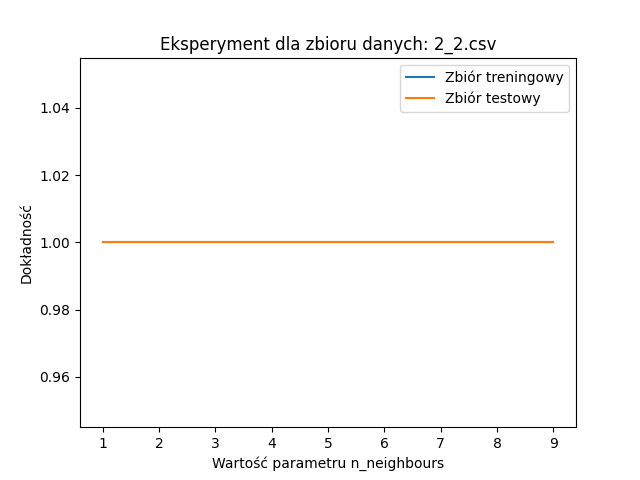
\includegraphics[width=\linewidth]{img/exp_2/knn/2_2/accuracy.png}
        \caption{Dokładność}
    \end{subfigure}
    \\
    \begin{subfigure}[t]{\subfigwidth}
        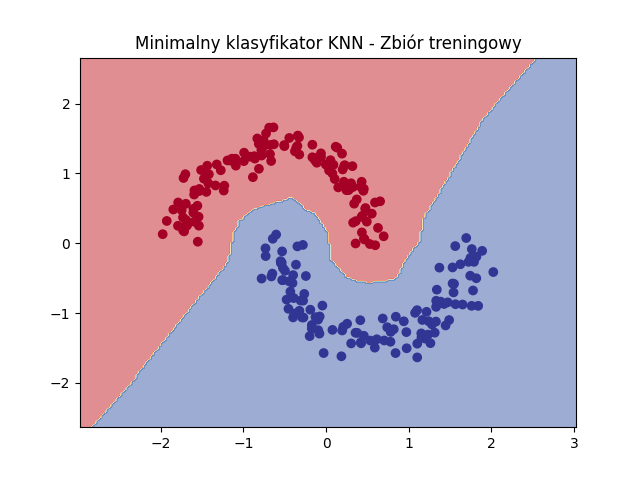
\includegraphics[width=\linewidth]{img/exp_2/knn/2_2/min/train_boundary.png}
        \caption{Min, train}
    \end{subfigure}
    \hfill
    \begin{subfigure}[t]{\subfigwidth}
        \includegraphics[width=\linewidth]{img/exp_2/knn/2_2/min/train_matrix.png}
        \caption{Min, train}
    \end{subfigure}
    \hfill
    \begin{subfigure}[t]{\subfigwidth}
        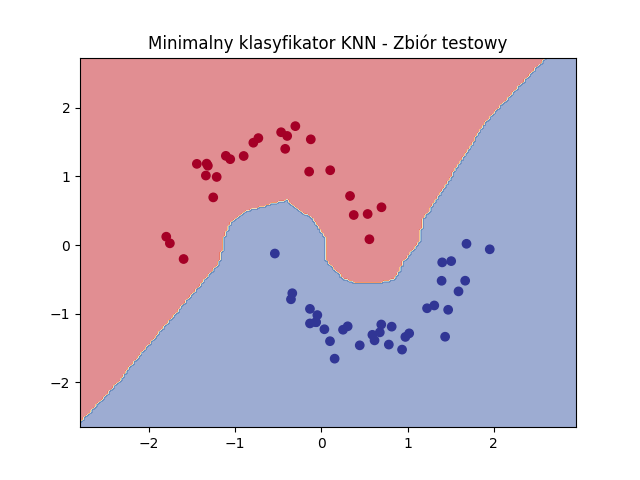
\includegraphics[width=\linewidth]{img/exp_2/knn/2_2/min/test_boundary.png}
        \caption{Min, test}
    \end{subfigure}
    \hfill
    \begin{subfigure}[t]{\subfigwidth}
        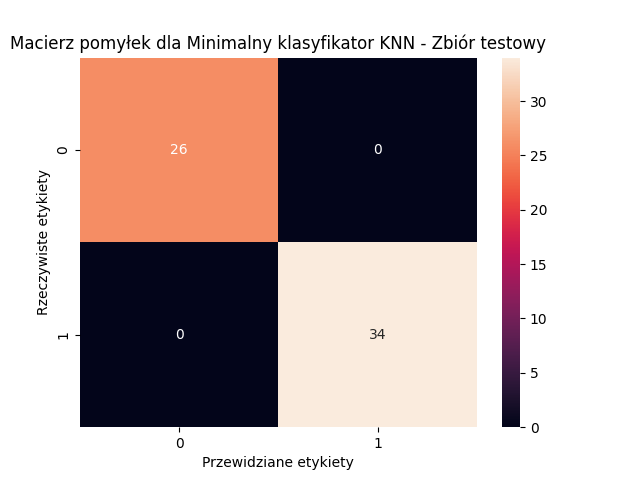
\includegraphics[width=\linewidth]{img/exp_2/knn/2_2/min/test_matrix.png}
        \caption{Min, test}
    \end{subfigure} 
    \\
    \begin{subfigure}[t]{\subfigwidth}
        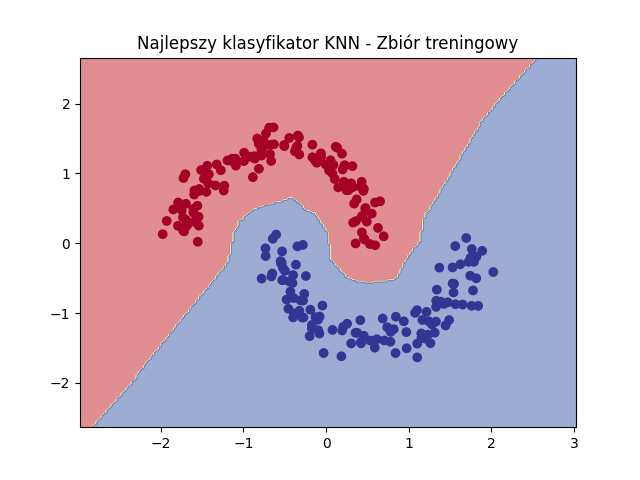
\includegraphics[width=\linewidth]{img/exp_2/knn/2_2/best/train_boundary.png}
        \caption{Best, train}
    \end{subfigure}
    \hfill
    \begin{subfigure}[t]{\subfigwidth}
        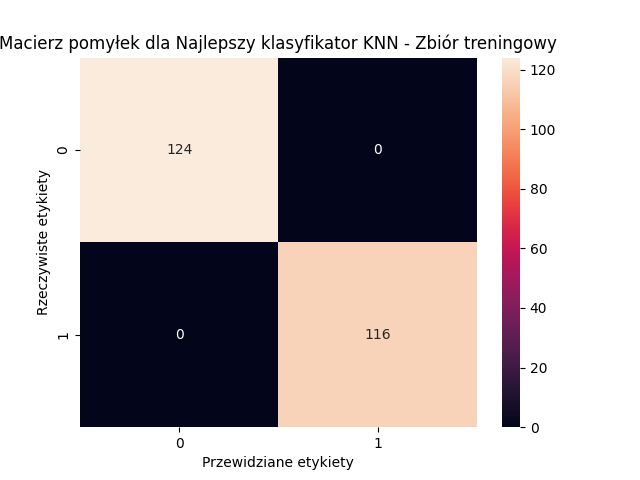
\includegraphics[width=\linewidth]{img/exp_2/knn/2_2/best/train_matrix.png}
        \caption{Best, train}
    \end{subfigure}
    \hfill
    \begin{subfigure}[t]{\subfigwidth}
        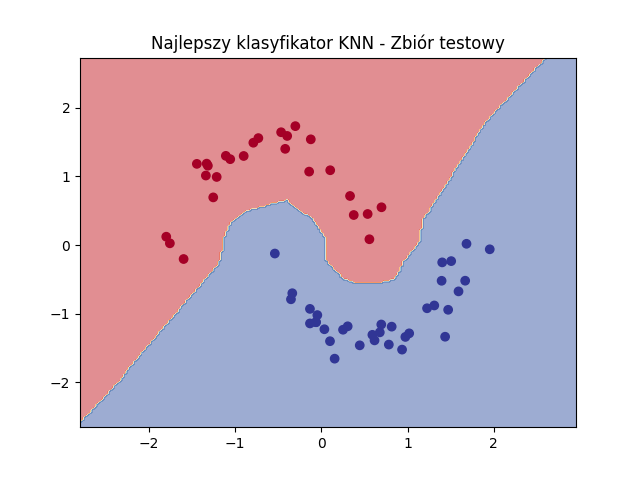
\includegraphics[width=\linewidth]{img/exp_2/knn/2_2/best/test_boundary.png}
        \caption{Best, test}
    \end{subfigure}
    \hfill
    \begin{subfigure}[t]{\subfigwidth}
        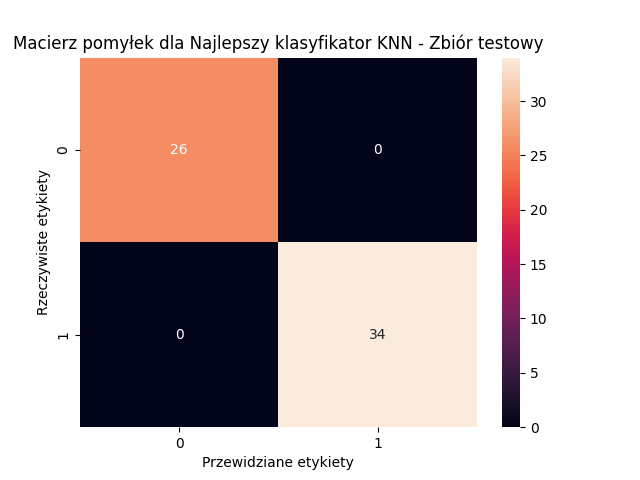
\includegraphics[width=\linewidth]{img/exp_2/knn/2_2/best/test_matrix.png}
        \caption{Best, test}
    \end{subfigure} 
    \\
    \begin{subfigure}[t]{\subfigwidth}
        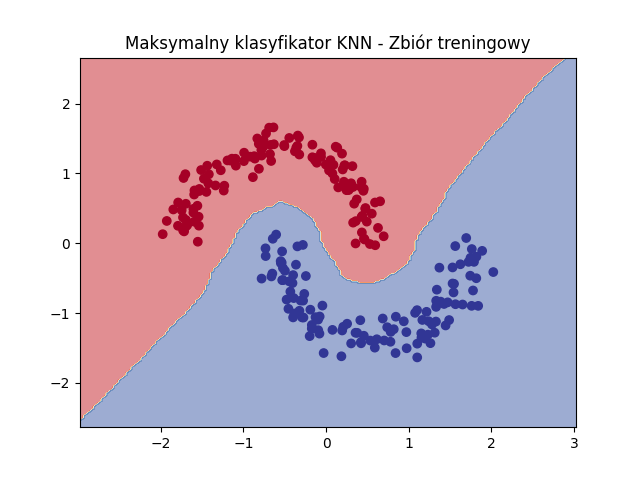
\includegraphics[width=\linewidth]{img/exp_2/knn/2_2/max/train_boundary.png}
        \caption{Max, train}
    \end{subfigure}
    \hfill
    \begin{subfigure}[t]{\subfigwidth}
        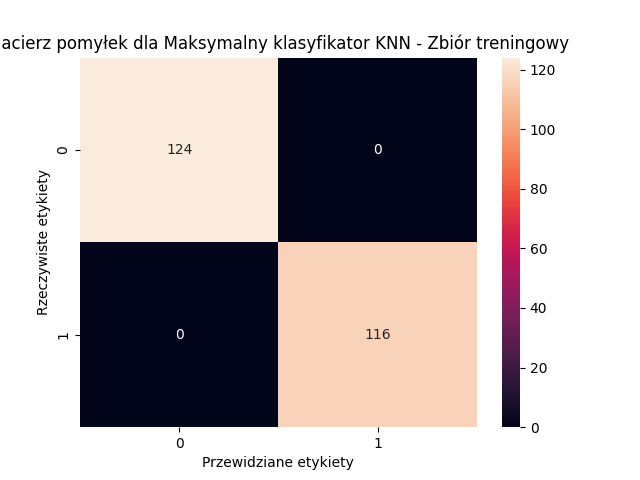
\includegraphics[width=\linewidth]{img/exp_2/knn/2_2/max/train_matrix.png}
        \caption{Max, train}
    \end{subfigure}
    \hfill
    \begin{subfigure}[t]{\subfigwidth}
        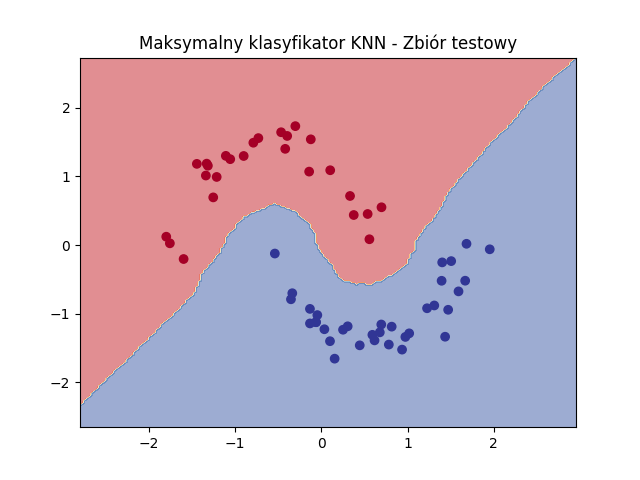
\includegraphics[width=\linewidth]{img/exp_2/knn/2_2/max/test_boundary.png}
        \caption{Max, test}
    \end{subfigure}
    \hfill
    \begin{subfigure}[t]{\subfigwidth}
        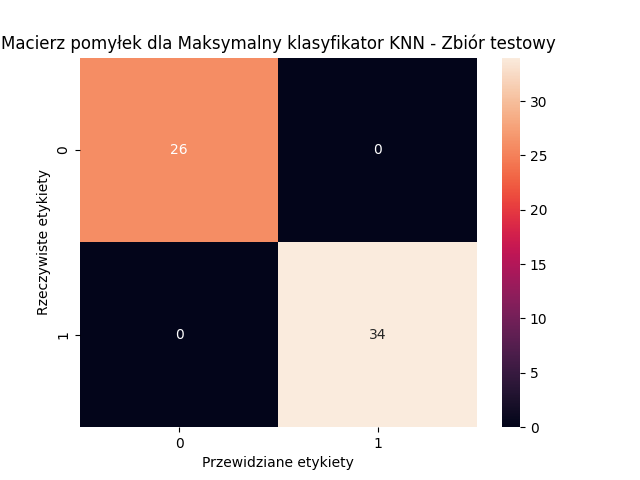
\includegraphics[width=\linewidth]{img/exp_2/knn/2_2/max/test_matrix.png}
        \caption{Max, test}
    \end{subfigure} 
    
    \caption{Wyniki dla zbioru 2\_2}
\end{figure}

\begin{figure}[H]\centering
    \begin{subfigure}[t]{\subfigwidth}
        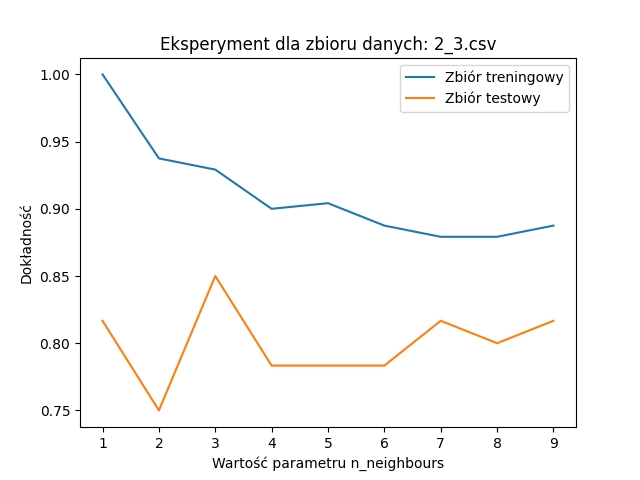
\includegraphics[width=\linewidth]{img/exp_2/knn/2_3/accuracy.png}
        \caption{Dokładność}
    \end{subfigure}
    \\
    \begin{subfigure}[t]{\subfigwidth}
        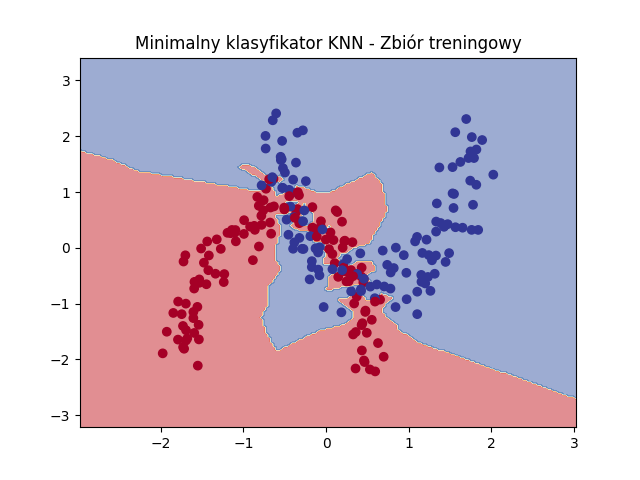
\includegraphics[width=\linewidth]{img/exp_2/knn/2_3/min/train_boundary.png}
        \caption{Min, train}
    \end{subfigure}
    \hfill
    \begin{subfigure}[t]{\subfigwidth}
        \includegraphics[width=\linewidth]{img/exp_2/knn/2_3/min/train_matrix.png}
        \caption{Min, train}
    \end{subfigure}
    \hfill
    \begin{subfigure}[t]{\subfigwidth}
        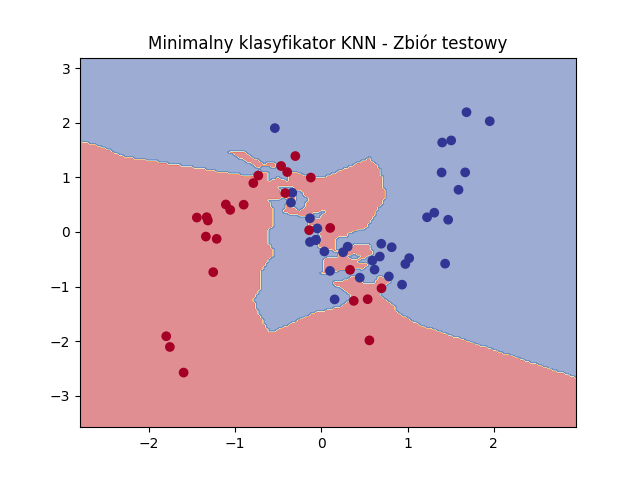
\includegraphics[width=\linewidth]{img/exp_2/knn/2_3/min/test_boundary.png}
        \caption{Min, test}
    \end{subfigure}
    \hfill
    \begin{subfigure}[t]{\subfigwidth}
        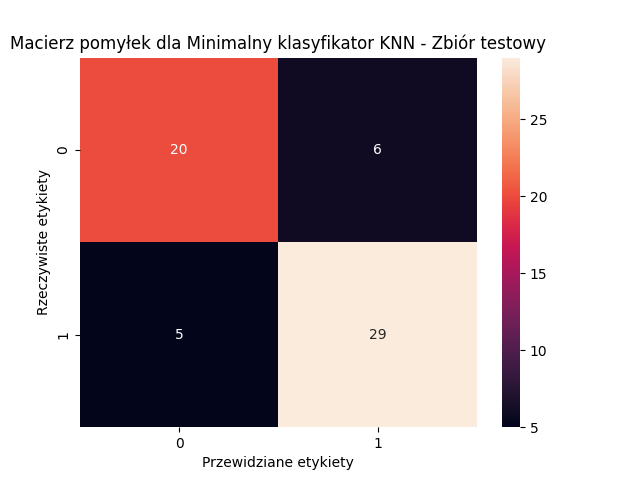
\includegraphics[width=\linewidth]{img/exp_2/knn/2_3/min/test_matrix.png}
        \caption{Min, test}
    \end{subfigure} 
    \\
    \begin{subfigure}[t]{\subfigwidth}
        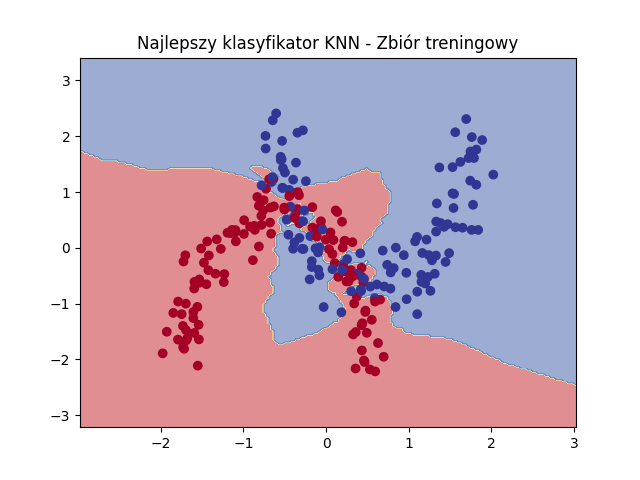
\includegraphics[width=\linewidth]{img/exp_2/knn/2_3/best/train_boundary.png}
        \caption{Best, train}
    \end{subfigure}
    \hfill
    \begin{subfigure}[t]{\subfigwidth}
        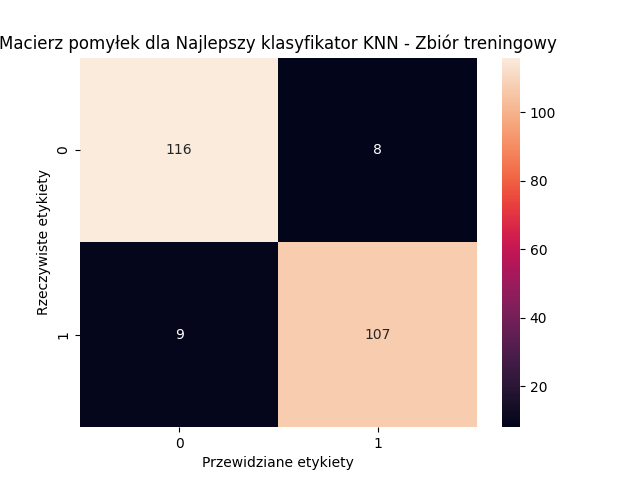
\includegraphics[width=\linewidth]{img/exp_2/knn/2_3/best/train_matrix.png}
        \caption{Best, train}
    \end{subfigure}
    \hfill
    \begin{subfigure}[t]{\subfigwidth}
        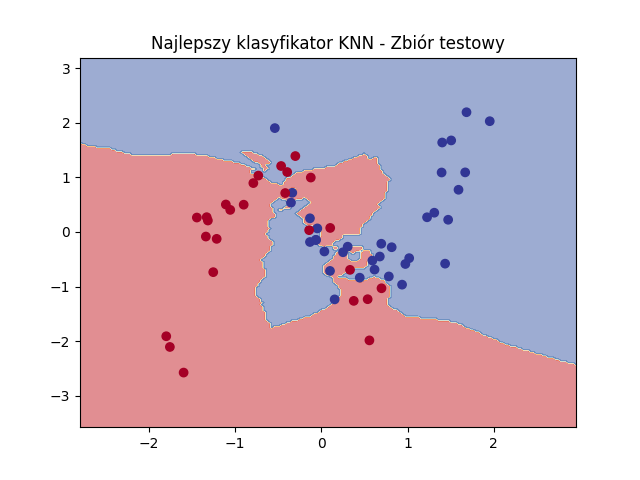
\includegraphics[width=\linewidth]{img/exp_2/knn/2_3/best/test_boundary.png}
        \caption{Best, test}
    \end{subfigure}
    \hfill
    \begin{subfigure}[t]{\subfigwidth}
        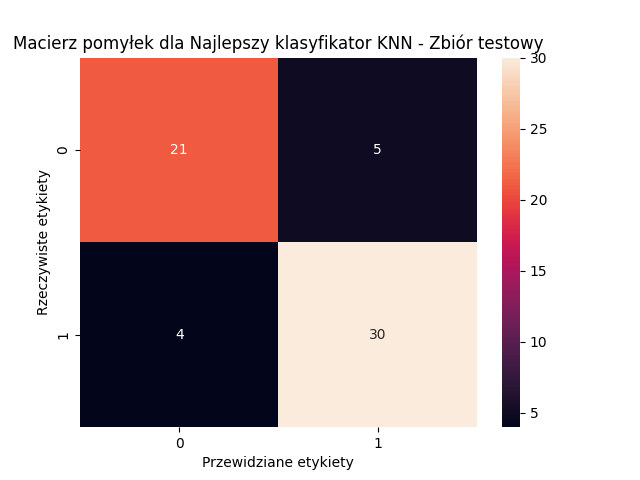
\includegraphics[width=\linewidth]{img/exp_2/knn/2_3/best/test_matrix.png}
        \caption{Best, test}
    \end{subfigure} 
    \\
    \begin{subfigure}[t]{\subfigwidth}
        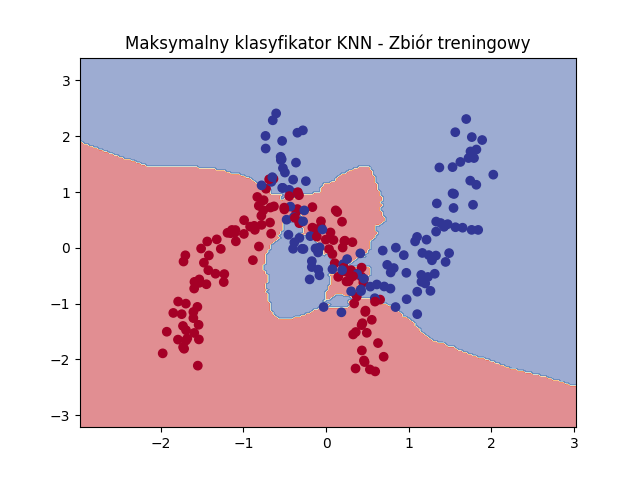
\includegraphics[width=\linewidth]{img/exp_2/knn/2_3/max/train_boundary.png}
        \caption{Max, train}
    \end{subfigure}
    \hfill
    \begin{subfigure}[t]{\subfigwidth}
        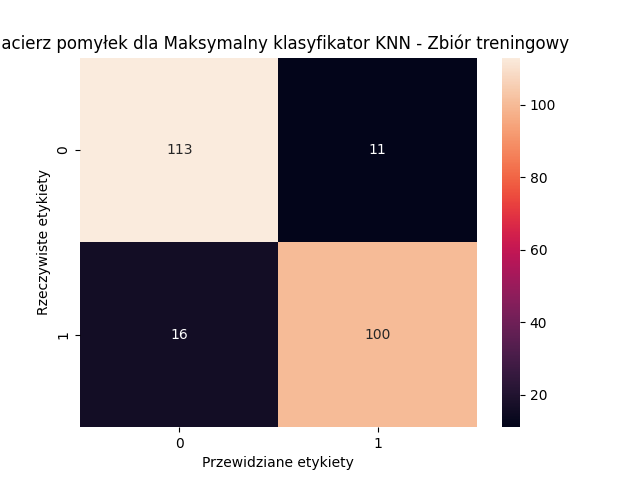
\includegraphics[width=\linewidth]{img/exp_2/knn/2_3/max/train_matrix.png}
        \caption{Max, train}
    \end{subfigure}
    \hfill
    \begin{subfigure}[t]{\subfigwidth}
        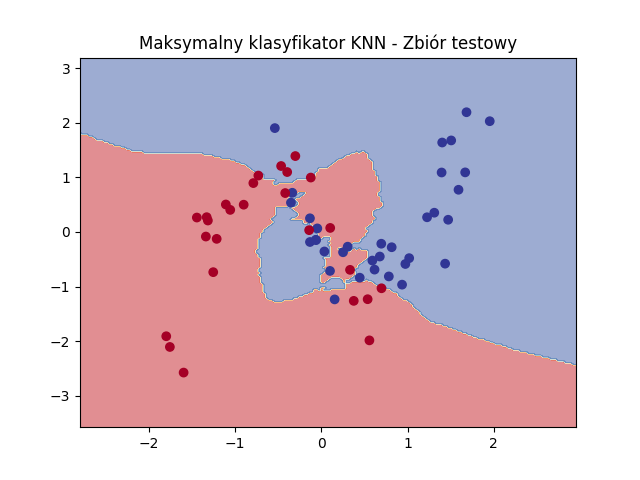
\includegraphics[width=\linewidth]{img/exp_2/knn/2_3/max/test_boundary.png}
        \caption{Max, test}
    \end{subfigure}
    \hfill
    \begin{subfigure}[t]{\subfigwidth}
        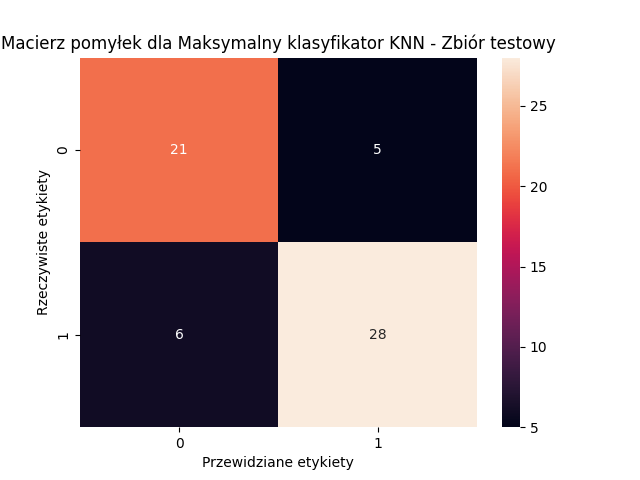
\includegraphics[width=\linewidth]{img/exp_2/knn/2_3/max/test_matrix.png}
        \caption{Max, test}
    \end{subfigure} 
    
    \caption{Wyniki dla zbioru 2\_3}
\end{figure}


\clearpage

3 strona --- Wyniki drugiego eksperymentu dla dwóch sztucznie wygenerowanych zbiorów danych 2\_2 i 2\_3 oraz metody SVM. Dla każdego zbioru należy pokazać wykres obrazujący zmianę wartości accuracy na zbiorach treningowym i testowym przy zmieniającym się parametrze C oraz wizualizacje przebiegu granicy decyzyjnej na zbiorach treningowym i testowym dla: najmniejszej, najlepszej (wartość accuracy na zbiorze testowym) i największej wartości tego parametru. Dodatkowo przy każdej wizualizacji należy pokazać jak wygląda macierz pomyłek. Wartości parametru C powinny się zmieniać wykładniczo, a na wykresie dobrze jest zastosować skalę logarytmiczną. 

\clearpage

4 strona --- Wyniki drugiego eksperymentu dla dwóch sztucznie wygenerowanych zbiorów danych 2\_2 i 2\_3 oraz sieci MLP. Dla każdego zbioru należy pokazać wykres obrazujący zmianę wartości accuracy na zbiorach treningowym i testowym przy zmieniającej się liczbie neuronów w warstwie ukrytej oraz wizualizacje przebiegu granicy decyzyjnej na zbiorach treningowym i testowym dla: najmniejszej, najlepszej (wartość accuracy na zbiorze testowym) i największej watości tego parametru. Dodatkowo przy każdej wizualizacji należy pokazać jak wygląda macierz pomyłek.

\clearpage

5 strona --- Wyniki trzeciego eksperymentu dla dwóch sztucznie wygenerowanych zbiorów danych 2\_2 i 2\_3 oraz metody K-NN. Dla każdego zbioru należy pokazać wykres obrazujący zmianę wartości accuracy na zbiorach treningowym i testowym przy zmieniającym się parametrze n\_neighbours oraz wizualizacje przebiegu granicy decyzyjnej na zbiorach treningowym i testowym dla: najmniejszej, najlepszej (wartość accuracy na zbiorze testowym) i największej wartości tego parametru. Dodatkowo przy każdej wizualizacji należy pokazać jak wygląda macierz pomyłek.

\clearpage

6 strona --- Wyniki trzeciego eksperymentu dla dwóch sztucznie wygenerowanych zbiorów danych 2\_2 i 2\_3 oraz metody SVM. Dla każdego zbioru należy pokazać wykres obrazujący zmianę wartości accuracy na zbiorach treningowym i testowym przy zmieniającym się parametrze C oraz wizualizacje przebiegu granicy decyzyjnej na zbiorach treningowym i testowym dla: najmniejszej, najlepszej (wartość accuracy na zbiorze testowym) i największej wartości tego parametru. Dodatkowo przy każdej wizualizacji należy pokazać jak wygląda macierz pomyłek. Wartości parametru C powinny się zmieniać wykładniczo, a na wykresie dobrze jest zastosować skalę logarytmiczną.

\clearpage

7 strona --- Wyniki trzeciego eksperymentu dla dwóch sztucznie wygenerowanych zbiorów danych 2\_2 i 2\_3 oraz sieci MLP. Dla każdego zbioru należy pokazać wykres obrazujący zmianę wartości accuracy na zbiorach treningowym i testowym przy zmieniającej się liczbie neuronów w warstwie ukrytej oraz wizualizacje przebiegu granicy decyzyjnej na zbiorach treningowym i testowym dla: najmniejszej, najlepszej (wartość accuracy na zbiorze testowym) i największej wartości tego parametru. Dodatkowo przy każdej wizualizacji należy pokazać jak wygląda macierz pomyłek.

\clearpage

8 strona --- Wyniki czwartego eksperymentu dla sztucznie wygenerowanego zbioru danych 2\_3 oraz sieci MLP. Dla rozważanego zbioru należy rozważyć przypadki z różną liczbą danych treningowych (parametr train\_size równy równy wartościom użytym odpowiednio w eksperymentach drugim i trzecim). Dla obu przypadków należy zaprezentować wykres zmian accuracy na zbiorach treningowym i testowym w kolejnych epokach oraz wizualizacje przebiegu granicy decyzyjnej na zbiorach treningowym i testowym dla epoki: zerowej (przed rozpoczęciem nauki), najlepszej (wartość accuracy na zbiorze testowym) i ostatniej (po zakończeniu nauki).
Dodatkowo w każdym z przypadków należy uruchomić proces treningu 10 razy z różnymi wagami początkowymi i w tabeli zamieścić wartości accuracy na zbiorze testowym i treningowym dla epoki: pierwszej (początek nauki), najlepszej (wartość accuracy na zbiorze testowym) i ostatniej (po zakończeniu nauki). W przypadku wartości najlepszej należy również podać numer epoki kiedy ją osiągnięto. Liczbę neuronów w warstwie ukrytej należy dobrać jako tą optymalną wynikającą odpowiednio z eksperymentów drugiego i trzeciego.

\clearpage

9 strona --- Opis wniosków z eksperymentów przeprowadzonych na sztucznie wygenerowanych zbiorach. W przypadku wszystkich ekseprymentów należy zwrócić uwagę na kształt uzyskiwanych granic decyzyjnych i związane z nim zdolności uogólniajace poszczególnych rodzajów klasyfikatorów (wpływ hiperparametrów) oraz wpływ liczby danych treningowych. W eksperymencie czwartym należy dodatkowo skupić się na zdolnościach uogólniających w kolejnych epokach nauki oraz na wpływie sposobu zaincjalizowania sieci. Wnioski powinny mieć charakter ogólny, pozwalający przenieść je na przypadek, w którym nie ma możliwości zwizualizowania danych. Każdy wniosek powinien być poparty odniesieniami do wyników przedstawionych na pierwszych czterech stronach raportu.

\clearpage

10 strona --- Opis działania analizowanych metod klasyfikacji w przypadku rzeczywistych zbiorów dnaych. Podczas tworzenia klasyfikatorów warto skorzystać z wniosków wyciągniętych podczas wcześniejszych eksperymentów. Uzyskane wyniki należy zaprezentować w zwartej formie (warto wykorzystać tabele i/lub wykresy), a wnioski należy poprzeć odwołaniami do tych wyników.

\end{document}